\documentclass{article}[18pt]
\ProvidesPackage{format}
%Page setup
\usepackage[utf8]{inputenc}
\usepackage[margin=0.7in]{geometry}
\usepackage{parselines} 
\usepackage[english]{babel}
\usepackage{fancyhdr}
\usepackage{titlesec}
\hyphenpenalty=10000

\pagestyle{fancy}
\fancyhf{}
\rhead{Sam Robbins}
\rfoot{Page \thepage}

%Characters
\usepackage{amsmath}
\usepackage{amssymb}
\usepackage{gensymb}
\newcommand{\R}{\mathbb{R}}

%Diagrams
\usepackage{pgfplots}
\usepackage{graphicx}
\usepackage{tabularx}
\usepackage{relsize}
\pgfplotsset{width=10cm,compat=1.9}
\usepackage{float}

%Length Setting
\titlespacing\section{0pt}{14pt plus 4pt minus 2pt}{0pt plus 2pt minus 2pt}
\newlength\tindent
\setlength{\tindent}{\parindent}
\setlength{\parindent}{0pt}
\renewcommand{\indent}{\hspace*{\tindent}}

%Programming Font
\usepackage{courier}
\usepackage{listings}
\usepackage{pxfonts}

%Lists
\usepackage{enumerate}
\usepackage{enumitem}

% Networks Macro
\usepackage{tikz}


% Commands for files converted using pandoc
\providecommand{\tightlist}{%
	\setlength{\itemsep}{0pt}\setlength{\parskip}{0pt}}
\usepackage{hyperref}

% Get nice commands for floor and ceil
\usepackage{mathtools}
\DeclarePairedDelimiter{\ceil}{\lceil}{\rceil}
\DeclarePairedDelimiter{\floor}{\lfloor}{\rfloor}

% Allow itemize to go up to 20 levels deep (just change the number if you need more you madman)
\usepackage{enumitem}
\setlistdepth{20}
\renewlist{itemize}{itemize}{20}

% initially, use dots for all levels
\setlist[itemize]{label=$\cdot$}

% customize the first 3 levels
\setlist[itemize,1]{label=\textbullet}
\setlist[itemize,2]{label=--}
\setlist[itemize,3]{label=*}

% Definition and Important Stuff
% Important stuff
\usepackage[framemethod=TikZ]{mdframed}

\newcounter{theo}[section]\setcounter{theo}{0}
\renewcommand{\thetheo}{\arabic{section}.\arabic{theo}}
\newenvironment{important}[1][]{%
	\refstepcounter{theo}%
	\ifstrempty{#1}%
	{\mdfsetup{%
			frametitle={%
				\tikz[baseline=(current bounding box.east),outer sep=0pt]
				\node[anchor=east,rectangle,fill=red!50]
				{\strut Important};}}
	}%
	{\mdfsetup{%
			frametitle={%
				\tikz[baseline=(current bounding box.east),outer sep=0pt]
				\node[anchor=east,rectangle,fill=red!50]
				{\strut Important:~#1};}}%
	}%
	\mdfsetup{innertopmargin=10pt,linecolor=red!50,%
		linewidth=2pt,topline=true,%
		frametitleaboveskip=\dimexpr-\ht\strutbox\relax
	}
	\begin{mdframed}[]\relax%
		\centering
		}{\end{mdframed}}



\newcounter{lem}[section]\setcounter{lem}{0}
\renewcommand{\thelem}{\arabic{section}.\arabic{lem}}
\newenvironment{defin}[1][]{%
	\refstepcounter{lem}%
	\ifstrempty{#1}%
	{\mdfsetup{%
			frametitle={%
				\tikz[baseline=(current bounding box.east),outer sep=0pt]
				\node[anchor=east,rectangle,fill=blue!20]
				{\strut Definition};}}
	}%
	{\mdfsetup{%
			frametitle={%
				\tikz[baseline=(current bounding box.east),outer sep=0pt]
				\node[anchor=east,rectangle,fill=blue!20]
				{\strut Definition:~#1};}}%
	}%
	\mdfsetup{innertopmargin=10pt,linecolor=blue!20,%
		linewidth=2pt,topline=true,%
		frametitleaboveskip=\dimexpr-\ht\strutbox\relax
	}
	\begin{mdframed}[]\relax%
		\centering
		}{\end{mdframed}}
\lhead{MCS - DMLA}


\begin{document}
\begin{center}
\underline{\huge The Basics of Graph Theory}
\end{center}
\section{What is a Graph?}
\begin{itemize}
	\item A mathematical model
	\item A representation of objects and relations between them
	\item The objects can be 'anything'
	\item The relations between pairs of anything
\end{itemize}
\section{Formal Definitions}
\subsection{Definitions}
A \textbf{graph} G is a pair $(V(G),E(G))$, where $V(G)$ is a \textbf{nonempty} set of \textbf{verticies}(or nodes) and $E(G)$ is a set of \textbf{unordered pairs} \{u,v\} with $u,v\in V(G)$ and $u\neq v$ called the \textbf{edges} of G.
\begin{itemize}
	\item V(G) can be infinite, but all our graphs will be finite
	\item If no confustion can arise we write $uv$ instead of $\{u,v\}$
	\item If the graph G is clear from the context, we write V and E instead of V(G) and E(G)
	\item It often helps to draw graphs
	\begin{itemize}
		\item represent each vertex by a point
		\item each edge by a line or curve connecting the corresponding points
		\item only endpoints of lines/curves matter, not the exact shape
	\end{itemize}
\end{itemize}
\section{A drawing of a graph}
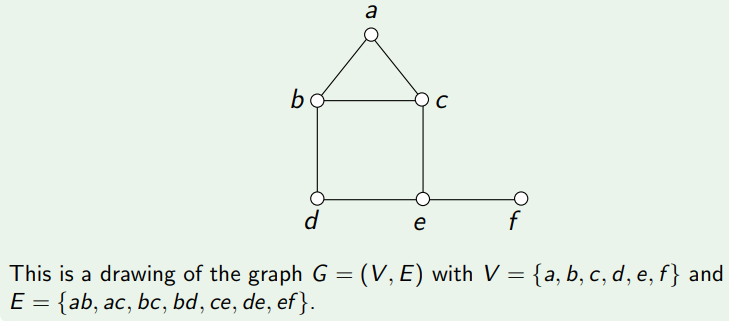
\includegraphics[scale=0.7]{drawing}
\section{Types of graphs}
\begin{itemize}
	\item \textbf{directed} graphs or \textbf{digraphs} - edges can have directions
	\begin{itemize}
		\item The web graph: vertices are webpages and edges are hyperlinks
		\item the precedence graph: vertices are program statements, edges reflect execution order
		\item the influence graph: vertices are people in the group, edges mean "influences"
	\end{itemize}
	\item multigraphs - multiple edges are allowed between two vertices
	\begin{itemize}
		\item the air link graph - several different airlines can fly between two towns
	\end{itemize}
	\item pseudographs - edges of the form $uu$, called loops are allowed
	\begin{itemize}
		\item region pseudograph in computer graphics: Vertices are connected regions edges mean "can get from one to the other by crossing a fence"
	\end{itemize}
	\item vertex or edge weighted graphs - vertices and/or edges can have weights
	\begin{itemize}
		\item the road map graph: weights on edges 
	\end{itemize}
\end{itemize}
By default, all our graphs are \textbf{simple undirected} graphs, that is, the above things are not allowed
\section{More examples of graph models}
Graphs can be useful to express \textbf{conflicting} situations between objects
\begin{itemize}
	\item vertices - base stations for mobile phones, Edges: overlapping service areas
	\item vertices - traffic flows at a junctions, Edges: conflicting flows
\end{itemize}
Graphs can be useful for \textbf{analysing strategies} and \textbf{solutions}
\begin{itemize}
	\item vertices: states in a game, edges: transitions between states
	\item vertices: steps in a solution, Edges: transitions between steps
\end{itemize}
\section{Terminology}
\subsection{Definitions}
Let G be a graph and $uv$ cn edge in it. Then
\begin{itemize}
	\item u and v care called endpoints of the edge $uv$
	\item u and v are called neighbours or adjacent vertices
	\item $uv$ is said to be incident to u (and to v)
	\item if $vw$ is also an edge and $w\neq u$ then $uv$ and $vw$ are called adjacent
\end{itemize}
\subsection{Definitions}
Let $G=(V,E)$ be a graph. The \textbf{neighbourhood} of a vertex $v\in V$, notation $N(v)$, is the set of neighbours of v i.e., $N(v)=\{ u\in V| uv\in E\}$.\\
The \textbf{degree} of a vertex $v\in V$ notation deg(v), is the number of neighbours of v i.e. $deg(v)=|N(v)|$\\
With $\delta(G)$ or $\delta$ we denote the \textbf{smallest degree} in G, and with $\Delta(G)$ or $\Delta$ or the \textbf{largest degree}\\
A vertex with degree 0 will be called an \textbf{isolated vertex}\\
A vertex with a degree 1 an \textbf{end vertex} or a \textbf{pendant vertex}
\subsection{Definition}
A subgraph $G'=(V',E')$ of $G=(V,E)$ is a graph with $V'\subseteq V$ and $E'\subseteq E$; this subgraph is called \textbf{proper} if $G'\neq G$ and spanning if $V'=V$
\section{First theorem in Graph theory}
Can you guess the relationship between the sum of the degrees of the vertices of a graph G and the number of edges of G
\subsection{Theorem(Handshaking Lemma)}
$$\text { Let } G = ( V , E ) \text { be a graph. Then } \sum _ { v \in V } \operatorname { deg } ( v ) = 2 | E |$$
This is useful for proving that a graph cannot exist
\subsection{Proof}
Every edge has two endpoints and contributes one to each of their degrees, so contributes two to the sum of the degrees of all the vertices of V
\section{Some graph classes}
Some graphs appear so often they have special names
\subsection{$P_3$}
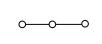
\includegraphics[scale=1.5]{p3}\\
This is denotes an $P_3$ and in general we define $P_n$ as a path on n vertices i.e. a graph with vertex set $\{v_1,v_2,...,v\}$ and edge set $\{v_1v_2,v_2v_3,...,v_{n-1}v_n\}$ So $P_n$ has n-1 edges
\subsubsection{Definition}
A path in a graph G is a subgraph of G which is $P_k$ for some integer $k\geqslant 1$. This notion is called a \textbf{simple path}
\subsection{$C_4$}
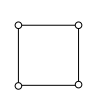
\includegraphics[scale=1.5]{c4}\\
In general a cycle $C_n$ on n verticies is defined similarly as a $P_n$, but with an additional edge between $v_n$ and $v_n$. So $C_n$ has n edges
\subsubsection{Definition}
A cycle in a graph G is a subgraph of G which is a $C_k$ for some integer $k\geqslant 3$. This notion is called a \textbf{simple circuit}
\subsection{$K_{p,q}$}
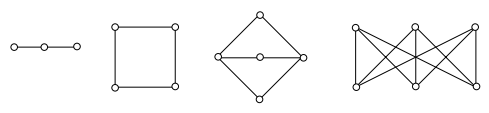
\includegraphics[scale=1.4]{kpq}\\
All four of these graphs can be described as $K_{p,q}$: a graph consisting of two disjoint vertex sets on p and q vertices and all the edges between the two vertex sets. So $K_{p,q}$ has $p\cdot q$ edges
\subsubsection{Definitions}
$K_{p,q}$ is called a \textbf{complete bipartite} graph. So a graph is bipartite iff we can partition its vertex set into two sets such that every edge has endpoints in each set
\subsection{Definition}
A \textbf{complete} graph on n vertices, denote by $K_n$ contains all the possible edges between pairs of vertices.\\
A $K_n$ graph has $\binom{n}{2}=\frac{1}{2}n(n-1)$
\subsection{Definition}
The (n dimensional) hypercube or n cube $Q_n (n\geqslant 1)$ is the graph with
$$V=\{(e_1,...,e_n)|e_i\in\{0,1\} (i=1,...,n) \}$$
in which two vertices are neighbours iff the corresponding rows differ in exactly one entry
\subsubsection{Example}
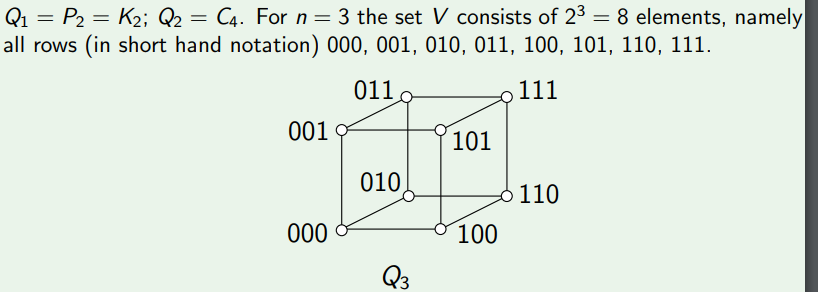
\includegraphics[scale=0.7]{n_dimension}
\section{More on n cubes}
\subsection{Theorem}
All n cubes are bipartite
\subsection{Proof}
\begin{itemize}
	\item We give a bipartition of the vertex set of the n cube
	\item Let $V_1$ contain all the vertices with an odd number of 1s
	\item Let $V_2$ contain all vertices with an even number of 1s
	\item This is clearly a partition of V into two disjoint sets
	\item It is easy to see that each edge has one endpoint in each of the sets
	\item So it proves that all n-cubes are bipartite
\end{itemize}

\section{Questions}
$p_n$ is only k regular for $p_2$\\
$c_n$ is k regular\\
$K_{p,q}$ is only k regylar for p=q\\
$Q_n$ is k regular\\
\\
\\
$p_n$ is bipartite\\
$C_n$ is bipartite only for even n\\
\\
\\
In $Q^n$ the number of verticies is $2^n$ and each has $n$ connections. The number of edges is $n\times 2^{n-1}$





\end{document}